\newcommand{\todoPorovani}[1]{
    \subsection{Architektura #1, možnosti konfigurace}
        \todo{Jaké má #1 části, jak se to deployuje, externí závislosti\ldots}\blind[4]
    \subsection{Rozšiřitelnost}
        \todo{Má #1 nějaké pluginy, dá se pro to scriptovat, jak je to bezpečné a jednoduché?}\blind[3]
    \subsection{Zabezpečení}
        \todo{Jaké jsou historická CVE? Jaká je izolace klientů? Co aplikace potřebuje za přístupy?}\blind[3]
    \subsection{Dostupnost}
        \todo{Může #1 běžet ve víc replikách? Jak se dělá upgrade? Jak stabilní to je?}\blind[3]
    \subsection{Integrace}
        \todo{Integrace #1, oznámení na GitHub/GitLab/Bitbucket/\ldots}\blind[2]
        \todo{Možnosti deploy z #1 do cílového systému; k8s, sftp, openstack, \ldots}\blind[5]
    \subsection{Praktické nasazení projektů}
        \subsubsection{Projekt 1}
            \todo{Popsat deploy projektu 1 z #1}\blind[2]
        \subsubsection{Projekt 2}
            \todo{Popsat deploy projektu 2 z #1}\blind[2]
        \subsubsection{Projekt 3}
            \todo{Popsat deploy projektu 3 z #1}\blind[2]
}

\chapter{Porovnání}
    V této práci se budu soustředit na systémy pro webové aplikace. To jsou především Javascript, Java, Python a PHP \cite{github-octoverse-languages}. Přesto že se \CI většinou nelimitují na konkrétní jazyky, vyhnu se při porovnání systémům primárně pro mobilní a desktopové aplikace. Dále se nebudu věnovat úzce zaměřeným proprietárním systémům (jako jsou například \textit{Visual Studio Team Services}, \textit{TeamCity}, \ldots).

    Přestože je hodně systémů prodáváno jako \CICD, podporují většinou pouze \CI část (primárně testování) a v nejlepším případě nějakou formou umožňují sledovat a spouštět nasazení aplikace. To je případ Jenkins, GitLab, Drone a dalších \cite{ellingwood-cicd-list}. To souvisí s tím, že pro komplexní \CD systém je nezbytná úzká integrace s hostitelskými servery -- hlavní komponenty které \CD konfiguruje jsou networking a potažmo DNS, \HTTP web servery, můžou nastavovat load balancery případně jiné části infrastruktury jako jsou databáze atd.

    Budu porovnávat zlášť \CI a \CD systémy; ukázalo se, že neexistuje jeden systém, který by kvalitně zvládat zastoupit obě role. U testovacích systémů, které se honosí podporou \CD vypíchnu co opravdu mají implementované a co jim chybí.

    \section{Metodika porovnávání \CI systémů}
        U každého systému se nejprve seznámím s aktuální dokumentací. \CI systémy provozované pouze jako \glstext{SaaS} (\textit{Software as a Service}) budu muset testovat v cloudu. Pokud systém nabízí self-hosted variantu, zprovozním ji na lokálním virtuálním serveru. Pro systémy s oficiálním kontejnerem budu systém spouštět v Dockeru. V případě, že systém má několik oficiálních variant instalace a nabízí jinou funkcionalitu (to je případ GitLabu), nainstaluji a otestuji systém několikrát. Všechny instalace budou nascriptované a opakovatelné. Technickou část práce netýkající se přímo daných \CI systémů popisuji \pfxref{v příloze}{ch:implementace}.

        Na instalovaných systémech pak provedu základní nezbytné nastavení: to bude pravděpodobně konfigurace veřejné \glstext{URL}, případně portů. \todo{další?} Bez dalšího nastavení zhodnotím zvlášť aplikační dostupnost za provozu a za správcovských úkonů: samostatně pro pro aktualizace \CI systému a pro rekonfiguraci. Tím se dozvím, jestli se lze spolehnout na výchozí nastavení dodavatele. Dostupnost budu měřit nástrojem \code{siege} \ref{fulmer-siege}. Jde o podobný nástroj jako je Apache \code{ab} \ref{apache-ab}, který navíc umí parsovat přijaté \glstext{HTML} a odesílat další požadavky na odkázané javascripty, kaskádové styly a další zdroje. Simuluje tak lépe chování uživatelů s webovým prohlížečem. Dostupnost budu testovat kontinuálními požadavky bez prodlev (volba \code{--benchmark}) s 10 uživateli (\code{--concurrent=10}). Výsledkem testu je počet selhaných požadavků, měřených podle \HTTP kódu odpovědi. Ideální výsledek je 0 selhaných požadavků. Dostupnost za klasického provozu aplikace budu měřit po dobu 15 minut. U administrátorských úkonů budu dostupnost měřit po celou dobu úkonu, která se bude lišit.

        Následně nakonfiguruji systém tak, aby měl co nejlepší možnou dostupnost a opět zopakuji testy na dostupnost.
        \todo{Co se pro každý systém bude dělat (nastavovat, nasazovat).}
        \blind[4]

        \todo{Na jakých typových projektech tohle budu zkoušet.}

        \subsection{P1: Jednoduchá aplikace bez externích závislostí}
            Tato kategorie pokrývá výhradně statické weby. Aplikace může obsahovat dynamické části jako je například kontaktní formulář, ale samotné zpracování se děje mimo statickou aplikaci -- cílem formulářů může být například Google Form \cite{mccoy-google-form}, nebo jiné aplikace (ať už třetích stran nebo vlastní).

            Pro testování \CICD systémů jsem vytvořil jednoduchý statický projekt s nástrojem Jekyll \cite{jekyll}. Ten ze zdrojových souborů které se skládají hlavně z Markdown textů \cite{markdown}, metadat a šablon generuje statické \HTML soubory. Dále umí kompilovat i styly, což jsem využil pro jednoduchý \code{scss} soubor. Na závěr každého buildu se všechny assety přemístí do složky podle aktuálního data. Tím je aplikace připravena pro nasazení současně se starší nebo novější verzí.

            \todo{tohle asi přesunout někam do teorie jak se dělá deploy}

            Při \CICD se typicky v repozitáři uchovávají pouze zdrojová data. Pro generátory statických webů to mohou být například soubory ve formátu Markdown a specifikace \HTML šablon, ze kterých se. Z těch se pak v rámci buildu na \CICD pipeline vygenerují výsledné \HTML soubory. Je vhodné, aby statické zdroje (JavaScripty, kaskádové styly, \ldots) byly vygenerovány do unikátní složky, například podle verze buildu nebo podle času. Samotné nasazení na produkční server pak lze udělat bez výpadku takto: nejprve je nutné nasadit nové statické zdroje. Ty mají unikátní názvy (nejlépe jsou v unikátně pojmenovanné složce), takže jejich nasazení nepřepíše současné soubory. Následně se přepíší \HTML soubory. Uživatelé kteří ještě načetli starou verzi načtou staré zdroje. \HTML soubory neexistující v nové verzi lze po uvážení z produkčního serveru odstranit. Není potřeba invalidovat cache, protože nové zdroje jsou pojmenované jinak než ty staré. Po uplynutí vhodného času lze staré zdrojové soubory ze serveru smazat.

            \todo{obrázek jak se dělá statický deploy když to chci mít bez výpadku, časový diagram}

            Pro vysokou dostupnost je vhodné použít víc než jeden server. V tom případě stačí nahrát nové zdroje na všechny servery a po bariéře přepsat všechna \HTML.

            \todo{obrázek pro HA}

            Při použití kontejnerů nelze snadno dosáhnout toho, aby v containeru byly nové a současně staré zdroje. Místo toho se problém přesune na nějakou vyšší vrstvu, například ingress controller. Ten může podle \HTTP kódu odpovědi rozhodnout, jeslti se pokusí přeposlat požadavek na jiný kontejner. Pokud uživatel stáhne \HTML z nové verze aplikace, ale request na \glstext{CSS} přijde na starý container a vrátí kód \textit{404 Not Found}, může ingress controller GET požadavek přeposlat na nový kontejner, kde soubor existuje. Alternativou je použití session affinity, ale to nemusí fungovat dobře \todo{rozepsat}. Nebo lze mezi ingress controller a kontejnery umístit nějakou cachující \HTTP vrstvu (HAProxy, Varnish), která prakticky v základním nastavení načte a uloží do paměti zdroje z obou verzí. Je pouze nutné ošetřit, aby HTML ze starých kontejnerů nepřepsalo \HTML z kontejnerů nových, což může rozhodnout například podle hlavičky Last-Modified-At.

            \todo{obrázek pro kontejnery}

            \todo{následující texty přesunout mimo P1}
            Uchovávání knihoven třetích stran (například JavaScriptové \glstext{NPM} \todo{abbr} moduly) je kontroverzní: Copes rozvážně nepreferuje ani jednu variantu \cite{copes-commit-npm} \todo{přidat další}.

            \todo{citace} Nevýhodou přidání závislostí do repozitáře je zvětšení repozitáře, což má negativní dopad na rychlost mnoha operací a podle druhu \CICD pipeline přímý dopad na rychlost nasazování. Další problém je znepřehlednění rozdílů mezi jednotlivými verzemi v systému a při nevhodném použití verzovacího systému to může velmi komplikovat merge operace.

            \todo{citace} Výhody verzování externích závislostí jsou mnohé. Při buildu \CICD pipeline nemusí stahovat zdroje mimo samostatného repozitáře, což zvyšuje dostupnost při výpadku cizí služby (klasické závislosti jsou GitHub, JavaScript balíčky \glstext{NPM}, pro Javu Maven central repository). Aplikace se vždy buildí s předem známými a neměnnými verzemi závislostí, takže i při nezamknutí verze balíčku se při vydání breaking change nic nerozbije (v \glstext{PHP} composer.json, v \glstext{NPM} package.json, pro Java Maven pom.xml). Tento problém lze alternativně také řešit verzováním lockfile pro daný balíčkovací systém (composer.lock, package.lock/yarn.lock, Maven lockfile nemá); problém ale může stále nastat, pokud na cizím úložišti někdo otagovanou verzi balíčku přepíše. To se může stát buď omylem nebo třeba s nekalými úmysly a spoléhání na cizí úložiště při buildu tak lze považovat za bezpečnostní riziko. Při verzování závilostí mohou všechny zdrojové soubory podléhat kontrole. Dále verzování řeší projekty smazané \cite{williams-left-pad}.

        \subsection{P2: Komplexní aplikace}
            V této kategorii uvažuji komplexní aplikace vyžadující relační databázi, případně další závislosti jako jsou např. fronta, key-value storage, mailer, služba na zpracování obrázků nebo generování faktur, nebo platební bráne. Na rozdíl od statických webů se tyto aplikace složitě testují. V případě databáze například stačí spustit pro testy nový databázový stoj a pro novou databázi spustit migrace. V případě platební brány která může od aplikace požadovat veřejně dostupnou url pro webhooks to může znamenat, že už samotný test vyžaduje nějakou úroveň nasazení aplikace. \todo {tohle přepsat, je to neohrabané}

            Pro testování jsem implementoval blog v PHP, konkrétně za použití frameworku Symfony \cite{symfony}. Aplikace při zpracování každého požadavku posílá dotazy na články do externí MySQL databáze. Dále komunikuje s key-value serverem Redis, kde spravuje session. Třetí závislost je API třetí strany: \code{mailgun.com}, které se používá pro posílání transakčních emailů.


        \subsection{P3: Aplikace distribuovaná jako kontejner}
            Aplikace v kontejneru mají stejné nároky na testovací prostředí jako aplikace v předchozí skupině a v rámci \CICD se liší pouze v buildu a nasazení.

            \todo{Popsat projekt 3}\blind[1]

    \section{Jenkins}
        \todoPorovani{Jenkins}
    \section{Concourse}
        \todoPorovani{Concourse}
    \section{Drone.io}
        \todoPorovani{Drone.io}

    \section{GitLab}
    GitLab je především systém pro správu repozitářů a vzniknul jako otevřená alternativa služby GitHub. Nabízí ale velmi kvalitní vlastní \CI a má nástroje podporující \CD. GitLab je poskytován jako \glstext{SaaS} a to jak v managed variantě, tak v placené self-hosted variantě. Existuje i fukčně velmi ořezaná self-hosted verze zdarma. Veřejné jádro je poskytované jako \textit{GitLab Community Edition}, placené části jsou vedeny jako \textit{GitLab Enterprise Edition}.

    Oficiálně GitLab podporuje celou řadu instalačních možností od balíčků pro klasické Linux distribuce, přes Docker kontejnery až po složitější šablony pro Kubernetes nebo OpenShift. Do podzimu 2018 byl GitLab distribuován jako monolitická aplikace, které se velmi obtížně škálovala a spouštěla distribuovaně v několika replikách. Podařilo se ale GitLab rozdělit na jednotlivé komponenty (gitaly: git repozitáře, gitlab-shell: HA api nad gitaly, mailroom: správa příchozích emailů, sidekiq, task-runner, unicorn: ruby webserver). Dále ma GitLab řadu externích závislostí: relační databázi (konkrétně PostgreSQL, podpora pro MySQL už neexistuje), key-value storage (Redis), úložitě pro objekty (AWS S3 nebo otevřená alternativa s kompatibilním api Minio). V oficiálním docker image, kterému říkají \textit{omnibus}, jsou všechny tyto závislosti přibalené. Nově vznikly separátní docker image pro každou GitLab službu zvlášť a šablony pro Kubernetes Helm, usnadnující jejich spuštění a konfiguraci.

    Protože jsou oba přístupy diametrálně odlišné, rozhodl jsem se nasadit GitLab jak v původním \textit{omnibus} variantě distribuované jako balíček pro Debian, tak ve variantě mikroslužeb v prostředí kontejnerů a porovnat obě varianty.

    \subsection{GitLab Omnibus}
        Instalace podle oficiální dokumentace je velmi jednoduchá. Jde jenom o přidání vlastního repozitáře a instalace balíčku \cite{gitlab-install-ubuntu}. Po instalaci je rovnou spuštěna celá aplikace a při přístupu na HTTP endpoint se rovnou zobrazuje dialog pro nastavení administrátorského hesla.

        Aplikaci lze konfigurovat na několika místech: z webového rozhraní, \code{gitlab.yml} a \code{gitlab.rb}). V každé části je bohužel trochu něco jiného. V rámci této práce jsem upravil konfiguraci v \code{gitlab.rb}, kde jsem nastavil externí \glstext{URL}, na kterou GitLab generuje externí linky (například v emailové komunikaci), počáteční heslo pro administrátora a především token, kterým se bude autentifikovat GitLab Runner obstarávající \CI.

    \subsection{GitLab mikroslužby}
        GitLab začal oficiálně na konci roku 2018 podporovat také nasazení do Kubernetes přes Helm \cite{gitlab-helm-chart}. Kubernetes je distribuovaný orchestrátor kontejnerů a Helm je balíčkovací aplikace. Každá komponenta GitLabu byla oddělena do samostatného docker obrazu a v Helm balíčku (\textit{Helm chart}) je pomocí Kubernetes zdrojů popsáno jak se dané kontejnery mají spouštět a jak jsou provázané. Teoreticky je možné kontejnery spouštět i ručně v jiném systému než Kubernetes, ale není to oficiálně podporované a neexistuje k tomu dokumentace.

        \todo{diagram}
        \missingfigure[figwidth=\columnwidth,figheight=7cm]{Architektura GitLab \label{pic:gitlab-architecture}}

        Hlavní výhody nasazení GitLabu přes mikroslužby jsou:
        \begin{itemize}
            \item Přehlednost. Administrátor přesně ví, jaké komponenty systém obsahuje. Jednotlivé části nejsou skryté v Omnibus balíčku, kde se těžko dohledávají logy.
            \item Metriky mohou přímo využívat exportery nasazené v clusteru. V Omnibus jsou k dispozici pouze metriky pro celý balík, nebo je musí další proces uvnitř exportovat. To je další komplexita a nekonzistence se zbytkem prostředí.
            \item Lepší škálovatelnost. Můžeme škálovat pouze některé komponenty. Navíc díky přesným metrikám můžeme škálovat vytížené komponenty dynamicky.
            \item Využití upstream služeb. Řada komponent, které GitLab využívá, jsou nezměněné aplikace třetích stran. To je například ElasticSearch, Redis a relační databáze. V Omnibus balíčku jsou přibalené; nelze je aktualizovat a pokud na to GitLab nemyslel, nelze je vyčlenit a použít externí službu. U mikroslužeb má administrátor plnou kontrolu nad tím, které služby nasadí a pro které například použije cloudovou managed variantu.
        \end{itemize}

        Instalace GitLabu jako mikroslužeb je oproti verzi Omnibus velmi komplikovaná. Vyžaduje minimálně uživatelskou znalost Kubernetes a velmi podrobnou znalost Helm. Dokumentace je zatím (k lednu 2019) nekompletní a hodně nastavení a jejich význam je nutné dohledávat v šablonách Helm chartu. Některé konfigurace nejsou podporovánu vůbec. Narazil jsem například na nutnost nakonfigurovat Redis clusteru s heslem \cite{gitlab-helm-issue-redis}. Například managed varianta od \glstext{AWS} podporuje přihlášení heslem pouze při použití \glstext{TLS} tunelu, protože bez něj se posílá heslo v plaintextu a nedává moc smysl vůbec heslo použít. To souvisí s tím, že GitLab mikroslužby jsou velmi nové; dá se očekávat, že čím víc firem bude takto GitLab nasazovat, tím lepší dokumentace a podpora pro různá prostředí vznikne.

    \subsection{GitLab \CI}
        \CI není přímo komponenta distribuovaná s GitLab, je ale dobře zaintegrovaná. Díky skvělému návrhu GitLab pouze vystavuje události na \glstext{API}. K API se může registrovat libovolné množství runnerů, které se periodicky \glstext{API} dotazují na nové práce ke spuštění \cite{gitlab-runner-registration}. Runner může běžet na stejném serveru jako GitLab, ale velkou výhodou je možnost spustit runner i na jiném vzdáleném serveru -- například pro mobilní aplikace se často používá Mac mini s macOS, které je pro kompilaci nezbytné. Při registraci runneru je možné ho přidělit pouze některým projektům podle tagu, nebo ho zveřejnit pro všechny projekty. \todo{přiděluje to podle tagu gitlab nebo si to rozhoduje runner?}

        Runner při získání práce z \glstext{API} má k dispozici soubor s definicí (obsah souboru \code{.gitlab-ci.yml} \cite{gitlab-runner-yaml}) a přístupové údaje k repozitáři. Architektura GitLab \CI se skládá z tzv. \textit{stages} (etapy) a \textit{jobs} (kusy práce) (obrázek \ref{pic:gitlab-ci-architecture}). Jeden push do repozitáře typicky vygeneruje jednu \textit{pipeline}, což je sada \textit{stages} a \textit{jobs} popsaná konfigurací \CI v daném commitu.

        \todo{diagram}
        \missingfigure[figwidth=\columnwidth,figheight=7cm]{Architektura GitLab \CI \label{pic:gitlab-ci-architecture}}

        \todo{rozepsat moznosti konfigurace: že to umi cache, dependencies z predchozich jobu, ze to jde vsechno pouze seriove a dependencies se nepouzivaji pro paralelizaci}\blind[1]

        V oficiální implementaci nabízí runner celou řadu možností, jak jednotlivé \textit{jobs} spouštět, tzv. \textit{executors} \cite{gitlab-runner-config}. Základní je \code{shell}, při kterém neexistuje prakticky žádná izolace procesů a čištění prostředí. Jakékoliv závislosti, které je potřeba instalovat do sytému, ovlivňují všechny ostatní procesy na stejném serveru. Procesy běží pod neprivilegovaným uživatelem \code{gitlab-runner}, takže je lepší potřebné závislosti nainstalovat předem administrátorem. Tento executor může bbýt vhodný pro dedikované prostředí pokud zajistíme, že tento server využívá pouze jeden projekt, případně pouze důvěryhodné nekolidující projekty. Velmi podobně funguje executor \code{ssh}, který místo na lokálním stroji spouští příkazy vzdáleně. Na cílovém stroji nejsou potřeba žádné závislosti (samozřejmě s výjimkou ssh serveru); v cloudovém prostředí může být praktické mít čisté virtuální stroje, na které se pak ssh runner připojuje. Dále lze ssh executor využít pro systémy, na kterých runner nemůže běžet lokálně. Velkou nevýhodou tohoto prostředí je nízká opakovatelnost. Jelikož se všechny joby mohou navzájem ovlivňovat a hostující systém se průběžně mění, starší joby které dřív končili úspěšně už nemusí fungovat. Ostatní executory tento problém do značné míry eliminují.

        Zbylé executory mají kompletní izolaci všech jobů. Možnosti \code{parallels} a \code{virtualbox} startují pro každý job nový virtuální stroj, z jednoho obrazu podle konfigurace runneru. Kontejnerizace jobů je nabízena v executoru \code{docker}: pro každý job je možné zvolit vlastní image. Varianta \code{kubernetes} je pro runner běžící v Kubernetes clusteru a vytváří pro každý job nový pod. Všechny tyto executory mají dobře opakovatelné joby. Pokud nezměníme obraz virtuálního stroje, případně pokud používáme stále stejný docker image, budou až na případné externí závislosti joby spuštěné identicky jako dřív.

        \label{sec:gitlab-ci-docker}
        Nastavení \CI se dále komplikuje při buildu Docker obrazů. Při použití většiny executorů máme dvě možnosti. První varianta je použít hostitelský Docker. U \code{shell} (a potažmo \code{ssh}) executoru stačí vyřešit oprávnění (typicky je potřeba přidat uživatele \code{gitlab-runner} do skupiny \code{docker}). U \code{docker} případně \code{kubernetes} executoru můžeme mountnout ovládací Unix socket \code{/var/run/docker.sock} do našeho kontejneru. Pro virtuální stroje by teoreticky šel socket mountnout také, ale když přijdeme o izolaci nemusíme pak \glstext{VM} používat vůbec. Nevýhodou tohoto řešení je, že všechny aplikace využívající \CI vidí obrazy a cache ostatních aplikací. Pokud se jedna z aplikací přihlásí do vzdáleného registru a stáhne nějaký soukromý obraz (\code{docker pull}), všechny ostatní aplikace tento obraz pak vidí a mohou ho číst i přesto, že nemají k vzdálenému registru oprávnění. Podobně jako při použití \code{shell} executoru tak musíme při sdílení Docker daemonu na \CI stavět pouze důvěryhodné aplikace.

        Druhou variantou buildu Docker obrazů je tzv. \textit{Docker in Docker} (\glstext{DinD}). To je Docker démon zabalený do Docker kontejneru. Při spuštění stále sdílí Linuxové jádro s hostitelským systémem, ale samotný Docker proces je izolovaný: má samostatný seznam procesů, vlastní limity a oddělenou build cache. \glstext{DinD} může být spuštěný právě pro jeden job. Ukázková specifikace pipeline pro Docker v kontejnerovém prostředí je popsána \pfxref{v kódu}{fig:gitlab-dind}.

        \begin{figure}[hb]
            \begin{minted}[frame=lines,framesep=2mm,linenos]{ruby}
services:
  - "docker:dind"

variables:
  DOCKER_HOST: "tcp://docker:2375"

build:
  stage: build
  script:
    - docker build --tag demo-build .
            \end{minted}
            \caption{Ukázkový soubor \code{.gitlab-ci.yml} pro nastavení \glstext{DinD}.}
            \label{fig:gitlab-dind}
        \end{figure}

        Při samostatně spuštěném \glstext{DinD} pro každý build máme perfektní izolaci všech klientů, ale přicházíme o některé výhody Dockeru, konkrétně o stažené obrazy a cache předchozích buildů. To je známý problém a GitLab ho bez úspěchu řeší už několik let \cite{gitlab-docker-artifact-caching}. Největší výhoda tohoto řešení je perfektní dostupnost: každá pipeline má vlastní Docker a případné aktualizace se dějí na úrovni změny obrazu v \code{.gitlab-ci.yml}. Přes GitLab mechanizmus pro cachování lze uložit Docker data a při dalším jobu je opět nahrát do nového Docker daemona \cite{patel-docker-cache}. Toto řešení je ale velmi pomalé. Obrazy včetně cache budou běžně kolem stovek megabajtů a zapisujeme je dokonce hned čtyřikrát: jednou na disk při exportu, potom do GitLab cache což je často externí objektové úložiště (jako je AWS S3) a po čtvrté při načítání do prázdného Dockeru. Pro aplikace s extrémně dlouhým buildem v řádu desítek minut to může být přínosné, ale pro typické webové aplikace na které se tato práce soustředí není toto řešení vhodné.

        Velmi úspěšně lze ale \glstext{DinD} provozovat jako dlouhožijící službu oddělenou od samotné \CI pipeline. Získáme tím tak výhody obou řešení a veskrze eliminujeme všechny nevýhody. Pro každou skupinu navzájem si věřících aplikací spustíme samostatný \glstext{DinD} proces. Ten může běžet na hostitelském serveru s \CI nebo libovolném externím. V daných pipeline specifikacích pak stačí neuvést \code{services: "docker:dind"} a nakonfigurovat proměnnou \code{DOCKER\_HOST} (například \code{tcp://group-7.external-docker.local:2375}). Každá skupina aplikací uvidí pouze svoje obrazy a bude mít persistentní cache. Nevýhodou tohoto řešení je vysoká komplexita. Je nutné nějakým způsobem zajistit, aby se k Docker socketu mohly připojit pouze autorizované aplikace. Na to je praktické použít nějakou pokročilou abstrakci, například Network Policies v Kubernetes. Samotná \glstext{ACL} logika může být v síťové vrstvě jako je například Weave, Contrail nebo Calico, nebo v samostatném dedikovaném firewallu.

    \subsection{Podpora \CD praktik}
        \todo{cd: manualni spusteni jobu, gitlab operations environments v placenem}\blind[1]
        \todo{že to umi nasazovani beta aplikaci, podpora kubernetes}\blind[1]
        \todo{review apps}

    \subsection{Open-source}
        \todo{popsat jak se ten projekt vyvyji a ze je nerealne tam neco mergnout, protoze to dela milion lidi a nikdo to nevede}\blind[1]

    \subsection{Rozšiřitelnost}
        \todo{Má gitlab nějaké pluginy, dá se pro to scriptovat, jak je to bezpečné a jednoduché?}\blind[1]

    \subsection{Zabezpečení}
        Podle \glstext{CVE} Details měl GitLab nejvíc kritické problémy -- hodnocené podle podle \glstext{CVSS} -- zjištěné v posledním roce (2018) \cite{cve-gitlab}. To může souviset s exponenciálním růstem, který zažili díky \code{\#movingtogitlab} a akvicizi firmou Microsoft \cite{gitlab-growth}. Není zatím jasné, jestli dramatický nárůst počtu uživatelů přilákal bezpečnostní analytiky, nebo jestli bezpečnostní problémy jsou výsledkem zrychleného vývoje a zhoršení kvality produktu.

        \todo{Jak dlouho trvá gitlabu opravit cve a zverejnit fix?}

        Správa problémů (\textit{issues}) u projektů na GitLabu má možnost vytvořit nový záznam v důvěrném režimu. Takové problémy jsou pak viditelné pouze pro správce repozitáře. To je vhodné pro \textit{responsible disclosure} (zodpovědné zveřejnění) bezpečnostních chyb. GitLab toto úspěšně používá i pro vlastní projekty.

        GitLab zavádí v kontextu \CICD nový pojem \textit{continuous security testing} (kontinuální bezpečnostní testování) \cite{gitlab-app-security}. Na rozdíl od testování po začlenění změn a nasazení, GitLab umožňuje každému vývojáři deploynout danou větev verzovacího systému do vlastního testovacího prostředí. To je znázorněno \pfxref{v diagramu}{fig:gitlab-review-cycle}.

        \begin{figure}[hb]
            \centering
            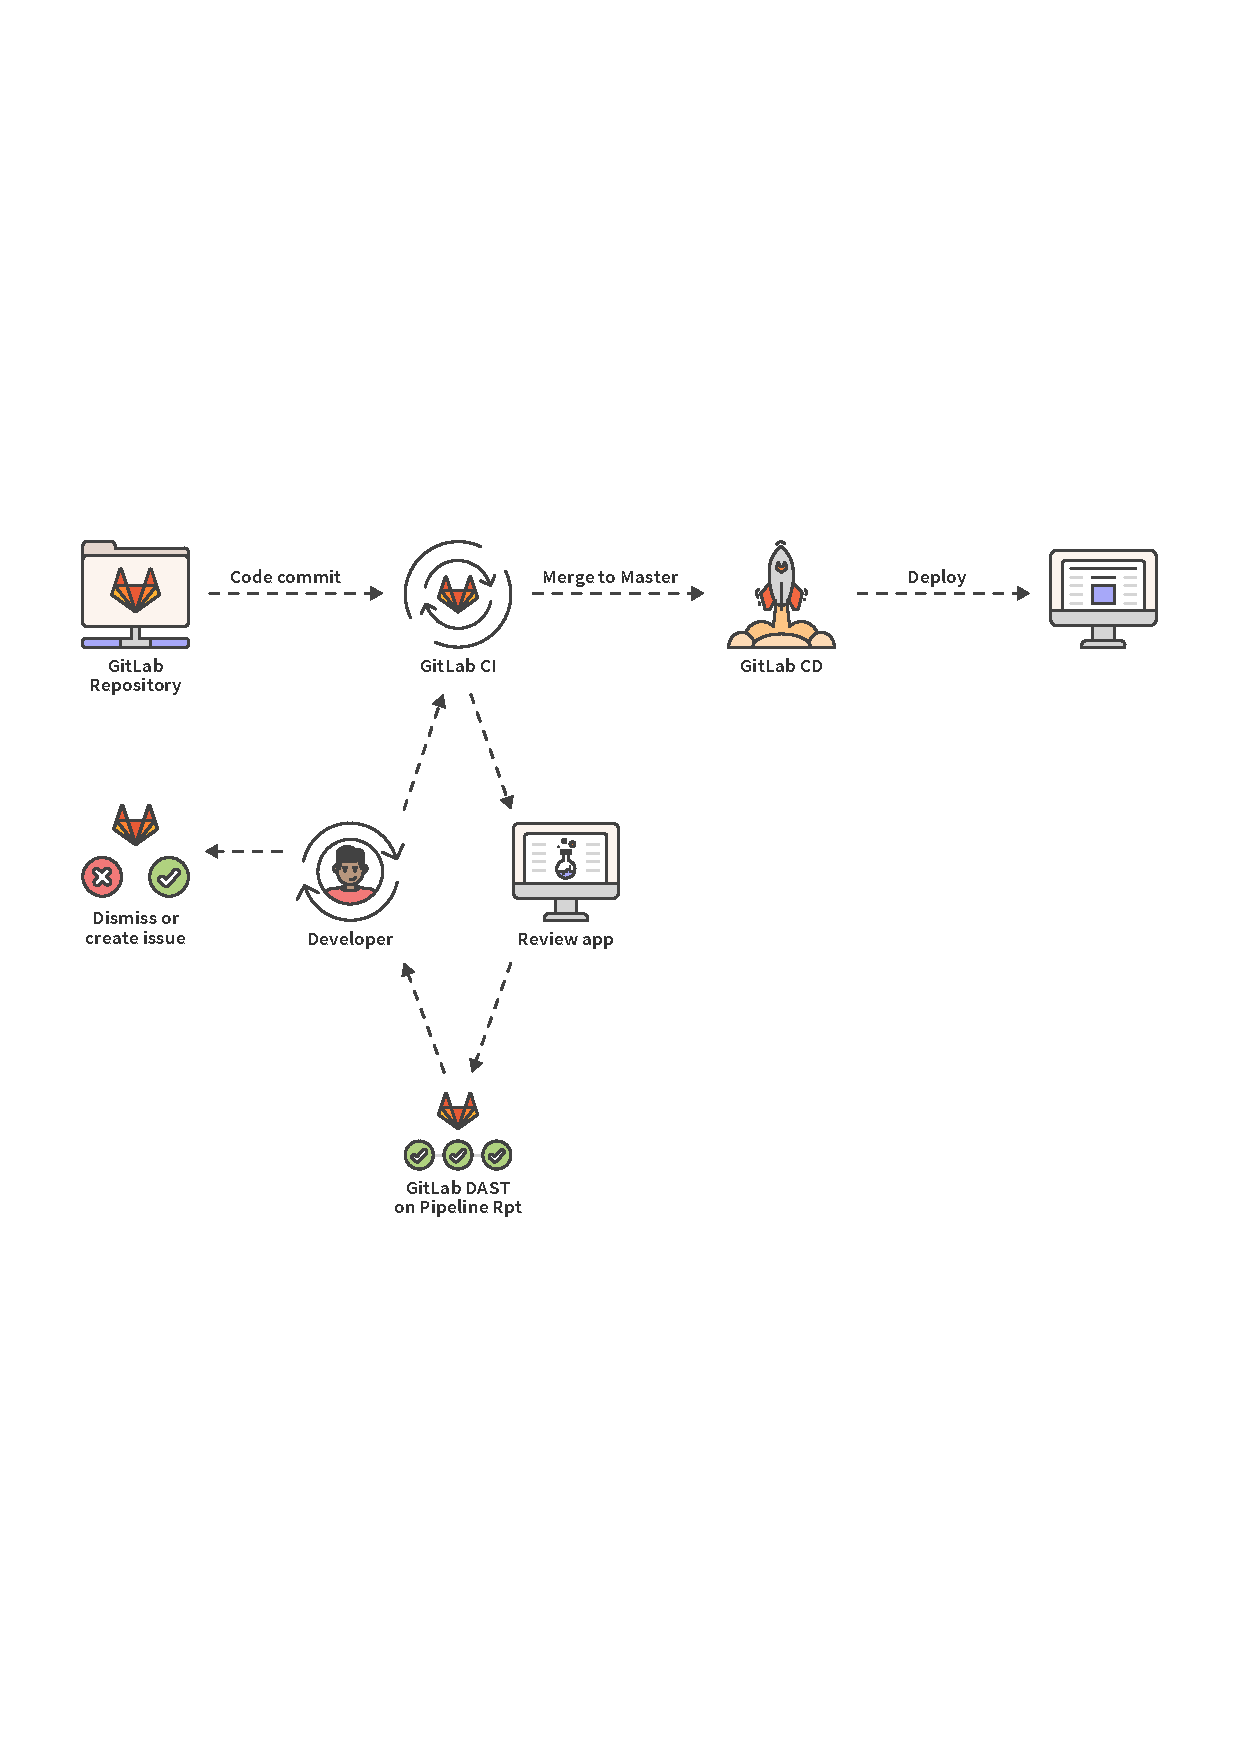
\includegraphics[width=\textwidth]{media/gitlab-review-cycle.pdf}
            \caption{Cyklus kontroly kvality aplikace GitLab s integrovaným \glstext{DAST} \cite{gitlab-app-security}. Vývojář může vyhodnotit bezpečnostní problémy před začleněním změň do sdíleného kódu.}
            \label{fig:gitlab-review-cycle}
        \end{figure}

        \todo{Jaké jsou historická CVE? Jaká je izolace klientů? Co aplikace potřebuje za přístupy?}\blind[1]

    \subsection{Dostupnost}
        \subsubsection{GitLab omnibus}
            Omnibus distribuce GitLabu, tedy balíček který obsahuje všechny komponenty, je primárně pro snadné nasazení a nepočítá se s tím, že by běžel s vysokou dostupností (\HA). Umožňují ale aktualizovat systém bez výpadku: doporučený postup je aktualizovat balíček, spustit databázové migrace a reloadnout webový frontend a konzumenty fronty \cite{gitlab-omnibus-update}. Důsledně se snaží dodržovat kompatibilitu napříč verzemi a databázové migrace dělají zpětně kompatibilní. V každém vydání nové verze jsou změny rozepsané a případné nekompatibility jsou znázorněny v tzv. \textit{upgrade barometer}.

            V základním nastavení nelze GitLab Omnibus replikovat. Některé komponenty lze ale vyčlenit. Nezbytné jsou PostgreSQL a Redis. Jediné co pak zbývá a sdílí se mezi replikami jsou samotné git repozitáře na souborovém úložišti. Vyzkoušel jsem, že GitLab Omnibus správně funguje ve víc replikách, když se vyčlení databáze a repozitáře se sdílí přes \glstext{NFS}. Jedná se ale o nezdokumentované nasazení a nemá oficiální podporu.

            Při nasazení ve víc replikách lze docílit 100 \% dostupnosti při aktualizaci na novější verzi.

        \subsection{GitLab microservices}
            Mikroslužby jsou obecně vhodné pro \glstext{HA} systémy:

            \begin{quote}
                [\ldots] each microservice in microservice architectures is operationally independent from others, and the only form of communication between services is through their published interfaces. This is fundamental since this allows one to change, fix or upgrade a microservice without compromising the system correctness, provided that the interfaces are preserved. \textit{Dragoni et al.~\cite{dragoni-microservices}}
            \end{quote}

            Klíčové komponenty GitLabu můžeme provozovat ve víc replikách a aktualizaci dělat pomocí rolling update, naprosto transparentně pro ostatní části systému. Některé komponenty jako jsou konzumenti fronty a manažer příchozích emailů můžeme dokonce aktualizovat s krátkým výpadkem, bez pozorovatelného dopadu pro uživatele.

            Správa stavových služeb je v distribuovaném systému nejkomplikovanější. GitLab jich bohužel používá celou řadu: relační databázi PostgreSQL, key-value storage Redis a vlastní služby Gitaly pro správu repozitářů. PostgreSQL s master-slave architekturou lze provozovat s vysokou dostupností použitím hot standby instance \cite{kim-postgres}. Redis také používá master-slave architekturu, ale dokáže si v případě výpadku sám zvolit v clusteru nový master díky komponentě Redis Sentinel \cite{redis-ha}. Tyto služby poskytovatelé cloudu nabízí i se správou, kde zodpovídají za dostupnost a některé aktualizace.

            Služba Gitaly je v oficiálním Helm chartu \glstext{SPOF}. Vystavuje \glstext{gRPC} \glstext{API} nad git repozitáři, se kterým pracuje většina ostatních komponent. Gitaly běží v jedné replice a je závislé na stavových datech na disku. Konzultoval jsem tento problém s oficiální podporou a je možné Gitaly provozovat nad \glstext{NFS} ve více replikách. Jde o kompromis mezi dostupností a rychlostí. Gitaly je z části limitováno propustností disku a \glstext{NFS} některé operace zpomalí.

\pfxref{Na diagramu}{pic:gitlab-architecture}
            \todo{todo popsat: vypsat komponenty a pak sepsat ze gitaly neni HA}

        \todo{Může gitlab běžet ve víc replikách? Jak se dělá upgrade? Jak stabilní to je?}\blind[2]

    \subsection{Integrace}
        \todo{Integrace gitlabu, oznámení na GitHub/GitLab/Bitbucket/\ldots}\blind[2]
        \todo{Možnosti deploy z gitlabu do cílového systému; k8s, sftp, openstack, \ldots}\blind[5]

    \subsection{Praktické nasazení projektů}
        \subsubsection{Projekt 1}
            Nastavení pipeline pro statický projekt není vůbec přímočaré. Z webového rozhraní jsem vytvořil projekt včetně repozitáře, v lokálním git repozitáři jsem nastavil přidělený remote a zdrojové kódy jsem nahrál na GitLab. Potom jsem ručně napsal konfiguraci pipeline v souboru \code{.gitlab-ci.yml}. Protože jsem GitLab runner nasadil s executorem \code{shell}, nainstaloval jsem předem do sdíleného prostředí nezbytné závislosti. Popis instalace Ruby, Gem a balíčků Jekyll a Bundler jsem popsal \pfxref{v příloze}{ch:implementace}. Konfigurace GitLab pipeline obsahuje značné množství klíčových slov, ale má vynikající webovou dokumentaci. Uvítal jsem také podporu schématu v \glstext{IDE} IntelliJ IDEA \cite{idea-gitlab-plugin}, bez kterého se těžko s JSON pracuje.

            Pipeline jsem specifikoval dvoukrokovou. V prvním kroku se generují výstupy a výsledky se archivují jako tzv.~artefakty. V kroku druhém  se tyto artefakty stáhnou a nahrají na webový server. Díky tomuto rozdělení lze na GitLabu deploy opakovat bez nutnosti znovu generovat všechny artefakty. To umožňuje mj.~velmi rychlý rollback a obecně přesun mezi verzemi.

            Implementoval jsem podporu pro GitLab review apps. Změny z větve \code{deploy/prod} se automaticky nahrávají do produkčního prostředí. Ostatní větve se nasadí pro dynamicky vygenerovaného prostředí a vývojář je má po kontrole možnost ručně vypnout.

            Při použití \code{docker} executoru je pipeline stejně jednoduchá, ale odpadá nutnost předem nastavit prostředí a není nutné řešit kolize závislostí napříč projekty. GitLab dokáže artifacts ukládat z kontejneru stejně jako v \code{shell} executoru.

        \subsubsection{Projekt 2}
            Pipeline pro dynamický komplexní projekt je překvapivě podobná, jako u statického projektu. Opět jsem vytvořil dvě hlavní stage: build a deploy. Hlavní rozdíl je v samotných příkazech pro sestavení, které jsem abstrahoval do \code{Makefile}. Protože využívám \code{shell} executor, předinstaloval jsem \glstext{PHP}, balíčkovací systém composer a další. To je bohužel správa kterou je potřeba dělat mimo konfiguraci pipeline.

            Review apps jsem navrhnul teoreticky, protože bez kontejnerů je implementace zbytečně složitá. U relační databáze (ve smyslu \glstext{RDBMS}) je potřeba vytvořit novou databázi, nakonfigurovat oprávnění pro nového uživatele aby nemohl ovlivnit ostatní (a hlavně produkční) databáze, nakonfigurovat aplikaci aby používala jiné databázové údaje a spustit migrace. Dále je potřeba po ukončení review app nějakým způsobem tuto databázi smazat. Velmi podobný postup je potřeba opakovat pro key-value storage, na které je aplikace také závislá.

        \subsubsection{Projekt 3}
            Opět jsme použil úplně stejnou pipeline jako pro předchozí dva projekty. Pro sdílení vystavěného docker obrazu jsem použil GitLab Container Registry, což je vestavěná služba. Registr je automaticky založený při vytvoření GitLab projektu. V build scriptu jsem provedl authentikaci \code{docker login}. Heslo jsem hardcodoval rovnou do scriptu. Alternativně může být nastaveno ve webovém rozhraní GitLabu a předáno do jobu jako proměnná prostředí (\code{env}). To má smysl hlavně pro veřejné projekty, kde nechceme heslo zveřejňovat; pak je ale nutné ohlídat, aby \CI job nemohl kdokoliv škodlivě upravit, spustit, a nechat si vypsat heslo do logu.

            Pro build aplikace se používá hostitelský docker démon. Celou řadu výhod a nevýhod a alternativní řešení jsem rozepsal \pfxref{v sekci o Dockeru}{sec:gitlab-ci-docker}.

            Pro spuštění aplikace na webovém serveru se nejprve nahraje soubor pro konfiguraci Docker Swarm stacku. Na webovém serveru se pak spustí přihlášení do registru a příkazem \code{docker stack deploy} se spustí a případně aktualizuje aplikace.

            U tohoto ukázkového projektu si použitím \code{docker} executoru moc nepomůžeme. Docker jako závislost musí být na hostitelském serveru předinstalovaný a pro zbytek se používají kontejnery.


    \section{GoCD}
        Systém GoCD vychází z projektu Cruise \cite{thoughtworks-gocd}. Oba projekty vznikly ve firmě ThoughtWorks, kde pracoval průkopník a zastánce praktik \textit{extrémního programování} M. Fowler \cite{fowler-go}. Fowler systém Cruise doporučoval ve známém článku o \CI \cite{fowler-ci}.

    \section{CircleCI, Semaphore, TravisCI}
        \todo{tohle asi spojit do jednoho jako velmi podobné PaaS, možná ověřit jestli je v tom nějaký velký rozdíl ve feature setu}
        \todoPorovani{TravisCI+PaaS}

    \section{možná Phabricator?}
        \todo{prozkoumat Phabricator}
    \section{-další-}
        IntelliJ TeamCity, Go CD, Atlassian Bamboo, Codeship, Codefresh, Wercker

    \section{nejake vlastni scriptiky}
        \todo{pokud malo dlouhe, porovnat nejake vlastni scriptiky}
        \blind[4]

    \section{Souhrn}
        \missingfigure[figwidth=\columnwidth,figheight=\textheight]{Tabulka s přehledem}
